\documentclass[a4paper]{article}

\usepackage[utf8]{inputenc}
\usepackage[T1]{fontenc}
\usepackage{textcomp}
\usepackage{listings}
\usepackage{lmodern}
\usepackage{amsfonts}
\usepackage{titling}
\usepackage{lipsum}
\usepackage[left=1in, right=1in, bottom=1in, top=1in]{geometry}
\usepackage{amsthm}
\usepackage{tcolorbox}
\usepackage{hyperref}
\usepackage{xcolor}
\usepackage{graphicx}
\usepackage{makeidx}
\usepackage{tikz}
\usepackage{cases}
\usepackage{apacite}
\usepackage{tkz-berge}
\usepackage{url}
\usepackage{tgtermes}
\usepackage{sectsty}
\usepackage{subcaption}
\usepackage{setspace}
\usepackage{float}
\usepackage{amsmath, amssymb}


% figure support
\usepackage{import}
\usepackage{xifthen}
\pdfminorversion=7
\usepackage{pdfpages}
\usepackage{transparent}
\usepackage{color}
\newcommand{\incfig}[2][1]{%
    \def\svgwidth{#1\columnwidth}
    \import{./figures/}{#2.pdf_tex}
}

%mathstyling
\theoremstyle{plain}
\newtheorem{thm}{Theorem}[section]
\newtheorem{lem}[thm]{Lemma}
\newtheorem{prop}[thm]{Proposition}
\newtheorem*{cor}{Corollary}

\theoremstyle{definition}
\newtheorem{defn}{Definition}[section]
\newtheorem{conj}{Conjecture}[section]
\newtheorem{exmp}{Example}[section]
\newtheorem{axiom}{Axiom}
\theoremstyle{remark}
\newtheorem*{rem}{Remark}
\newtheorem*{note}{Note}

\definecolor{darkgreen}{rgb}{0.0, 0.5, 0.0}

\pdfsuppresswarningpagegroup=1
\lstset{
tabsize = 4, %% set tab space width
showstringspaces = false, %% prevent space marking in strings, string is defined as the text that is generally printed directly to the console
numbers = left, %% display line numbers on the left
commentstyle = \color{darkgreen}, %% set comment color
keywordstyle = \color{blue}, %% set keyword color
stringstyle = \color{red}, %% set string color
rulecolor = \color{black}, %% set frame color to avoid being affected by text color
basicstyle = \small \ttfamily , %% set listing font and size
breaklines = true, %% enable line breaking
numberstyle = \tiny,
  frame=none,
  xleftmargin=2pt,
  stepnumber=1,
  belowcaptionskip=\bigskipamount,
  captionpos=b,
  escapeinside={*'}{'*},
  language=haskell,
  tabsize=2,
  emphstyle={\bf},
  showspaces=false,
  columns=flexible,
  showstringspaces=false,
  morecomment=[l]\%,
}
\begin{document}
	\begin{titlepage}
	\begin{center}
	\large
	University of Warwick \\
	Department of Computer Science \\
	\huge
	\vspace{50mm}
	\rule{\linewidth}{0.5pt} \\
	CS141 \\
	\vspace{5mm}
	\Large
	Functional Programming
	\rule{\linewidth}{0.5pt}
	\vspace{5mm}
	\begin{figure}[H]
	\centering
	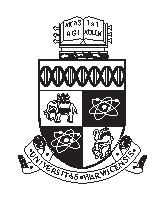
\includegraphics[width=0.4\textwidth]{crest_black.eps}
	\end{figure}
	\vspace{37mm}
	Cem Yilmaz \\
	\today
	\end{center}
	\end{titlepage}
	\newpage
	\tableofcontents
	\newpage
	\section{What is Functional Programming}
	\subsection{History}
	
	In 1928, David Hilbert posed the question "Given any true mathematical statement, is there an algorithm for verifying that it is true?". This is now known as the "Entscheidungsproblem", that is, the decision problem. E.g.
	\begin{align*}
		1 = 1 \\
		2 = 2 \\
		2 < 3 \\
		1 < 3
	\end{align*}
In 1931, Kurt Gödel came up with the paradox with the statement "This statement is not provable". If we assume not provable, there is a double negation which implies it is provable. This contradicts the assumption. If we assume true, we have a true statement that is not provable. This is called the incompleteness theorem. This answered the question that mathematics cannot answer every statement.\\
\begin{flushleft}
In 1936, Alonzo Church came up with $\lambda-$calculus as a system for describing algorithms. Kurt Gödel then believed that he can do better. He believed that some algorithms would not be able to be described with $\lambda-$calculus. Kurt then came up with a system of recursive functions. Alonzo Church then claimed that any algorithm that can be described using recursive functions can also be described using $\lambda-$calculus.  \\ 
\end{flushleft}
\begin{flushleft}
Alan Turing then came along and then came up with his own system of describing algorithms utilising Turing machines. However, he also showed that anything described using Turing machine could be described with $\lambda-$calculus. However, notice that despite these being different systems, they were also equivalent in describing algorithms. \\
\subsection{Today}

Today, programming as you know it, for example:
\[
\prod_{i=1}^{4} = 1 \times 2 \times 3 \times 4 
\] 
If we wanted to turn this to the roughly equivalent program in a language such as Java or C
\begin{lstlisting}[language = Java , caption ={Product in Java} , frame = trBL , firstnumber = last , escapeinside={(*@}{@*)}]
int x = 1;
for (int = 1; i <= 4; i++) {
	x *= i;
}
\end{lstlisting}
\begin{table}[H]
	\centering
	\caption{Table of results}
	\label{tab:results}
	\begin{tabular}{|c|c|}
		\hline
	Variable & Value \\
	\hline
	$x$ & $1$ \\
	$x$ & $2$ \\
	$x$ & $6$ \\
	$x$ & $24$ \\
	\hline
	\end{tabular}
\end{table}
\end{flushleft}
However, in a function language, we can express it as

\begin{lstlisting}[language = Haskell , caption={Product in Haskell} , frame = trBL , firstnumber = last , escapeinside={(*@}{@*)}]
product[1..4]
\end{lstlisting}
That is, product is a function. You can also expand this to be
\begin{lstlisting}[language = Haskell , caption={Expanded Product} , frame = trBL , firstnumber = last , escapeinside={(*@}{@*)}]
product[1,2,3,4] 
1 * product[2,3,4]
1 * 2 * product[3,4]
1 * 2 * 3 * product[4]
1 * 2 * 3 * 4
24
\end{lstlisting}
The definition of product function is rather simple:
\begin{lstlisting}[language = Haskell , caption={Product function} , frame = trBL , firstnumber = last , escapeinside={(*@}{@*)}]
product [n] = n -- Described in terms of 2 equations. First it checks if there a single item and returns it
product(n:ns) = n * product ns -- Takes the the first item in the list and keeps the rest
\end{lstlisting}
Let us now compare imperative programming with functional \\
\begin{flushleft}
\makebox[\textwidth][c]{
	\centering
	\label{tab:impvsfun}
	\begin{tabular}{|c|c|}
	\hline
	Imperative& Functional \\
	\hline
	Mutation of state & Reduction of expression \\
	Tell the computer how you want to do something & Tell the computer what you want to compute and let it work out how to do it \\
	Statements executed in order specified & Sub-expressions can often be evaluated in an arbitrary order \\
	Loops & Recursion \\
	\hline
	\end{tabular}
}
\end{flushleft}
\subsection{Programming Paradigms}
In history, there used to be a clear distinction between programming paradigms. However, today, this has changed. That is,
\begin{itemize}
	\item Java / C# are now multi-paradigm: They're imperative, object-oriented, functional, etc.
	\item Python, JavaScript, C++ have similarly multi-paradigm.
\end{itemize}
As such, learning functional programming will be useful as paradigms have blended together.
\subsection{What Haskell is good for}
\subsubsection{Web Services}

Furthermore, a particularly nice application to functional programming is that they're good at web services. 
\begin{itemize}
	\item Lots of cool frameworks for developing web applications
	\item Easy to embed domain-specific languages for routing, templates, etc.
	\item Servant: describe web service as a type, automatically generate client programs 
	\item One of the coursework assignments uses a web service written in Haskell to provide a browser-based interface
\end{itemize}
\subsubsection{Domain-specific language}

Domain-specific languages are also a thing. For example, you can write music in a Haskell library to describe music.
\begin{lstlisting}[language = Haskell , caption={Music in Haskell} , frame = trBL , firstnumber = last , escapeinside={(*@}{@*)}]
import Mezoo

v1 = d qn :|: g qn :|: fs qn :|:  g en :|: a en :|: bf qn :|: a qn :|: g hn
v2 = d qn :|: ef qn :|: d qn :|: bf_ en :|: a_ en :|: b_ qn :|: a_ qn :|: g_ hn

main = playLive (v1 :-: v2)
\end{lstlisting}
What's cooler is that if we try to compile, we would get an error that the composition is not harmonic, that is, if it does not sound good, it does not compile. In particular,
\begin{itemize}
	\item Major sevenths are not permitted in harmony: Bb and B\_
	\item Direction motion in a perfect octave is forbidden: Bb and B\_, then A and A\_
	\item Parallel octaves are forbidden: A and A\_, then G and G\_
\end{itemize}
\subsubsection{Games}
For example, the game magic cookies utilises functional reactive programming to describe its game logic. It is the same code across different platforms. It is also good for time-travel debugging.
\subsubsection{System Software}
\begin{itemize}
	\item XMonad: Window manager
	\item OS: Mirage (OCaml), House (Haskell) and more
\end{itemize}
\section{Haskell Files}
\subsection{Defining functions}
A haskell function looks like
\begin{lstlisting}[language = Haskell , caption={Function Definition} , frame = trBL , firstnumber = last , escapeinside={(*@}{@*)}]
triangle n = sum [1..n]
\end{lstlisting}
Function calls do not take brackets. We only use parentheses to set the order of operations. 
\subsubsection{Lambda Functions}
Recall Alonzho Church's $\lambda$-calculus terms are
\begin{align*}
	\lambda a. \lambda b. a b
\end{align*}
In haskell, we can write functions using with lambda notation:
\begin{lstlisting}[language = Haskell , caption={Lambda} , frame = trBL , firstnumber = last , escapeinside={(*@}{@*)}]
double = \x -> x*2
\end{lstlisting}
equivalent to
\begin{align*}
	\lambda x . x \times 2
\end{align*}
Notice this can also be defined as
\begin{lstlisting}[language = Haskell , caption={syntactic sugar} , frame = trBL , firstnumber = last , escapeinside={(*@}{@*)}]
double x = x * 2
double = \x -> x * 2
\end{lstlisting}
and so
\begin{lstlisting}[language = Haskell , caption={Syntactic sugaring} , frame = trBL , firstnumber = last , escapeinside={(*@}{@*)}]
foo x y = x * y
foo = \x -> \y -> x * y
\end{lstlisting}
\subsubsection{Arguments}

Let us see how this will be evaluate by computer step by step
\begin{lstlisting}[language = Haskell , caption={Step by step evaluation} , frame = trBL , firstnumber = last , escapeinside={(*@}{@*)}]
foo 5 6
-- (\x -> \y -> x * y) 5 6
-- (\y -> 5 * y) 6
-- 5 * 6
-- 30
\end{lstlisting}
If we put in a single argument instead,
\begin{lstlisting}[language = Haskell , caption={Partial function application} , frame = trBL , firstnumber = last , escapeinside={(*@}{@*)}]
foo 5
-- (\x -> \y -> x * y ) 5
-- (\y -> 5 * y)
\end{lstlisting}
Notice that we get back a function. This is called partial function application, and it is used everywhere in functional programming.
\subsection{Operators}
We are used to the standard mathematical operators such as $+$, $*$. If we want our own custom operators, we could implement them. Operator definitions look very similar to function definitions:
\begin{lstlisting}[language = Haskell , caption={defining operators} , frame = trBL , firstnumber = last , escapeinside={(*@}{@*)}]
x ^^^ y = max x y
\end{lstlisting}
We can also partially apply them and make them functions:
\begin{lstlisting}[language = Haskell , caption={Operator} , frame = trBL , firstnumber = last , escapeinside={(*@}{@*)}]
plusFive = (+ 5)
plus = (+)
(+) 5 6 
-- this would give 11 as it is equal to 5 + 6
\end{lstlisting}
The difference between operators and functions is that functions go before their arguments (prefix) and operators go between their arguments (infix). We are able to treat a function like an operator by enclosing it in backticks. We are able to treat an operator like a function by enclosing it in parentheses
\begin{lstlisting}[language = Haskell , caption={Operator Function relation} , frame = trBL , firstnumber = last , escapeinside={(*@}{@*)}]
5 `max` 6
-- gives an answer of 6
(*) 5 6
-- gives an answer of 30
\end{lstlisting}
Note that the number of argument stays the same, i.e., you cannot put 3 arguments into $(*)$ function.
\subsection{Pattern Matching}
We can change behaviour depending value of arguments. One way to do this is using if statements:
\begin{lstlisting}[language = Haskell , caption={Factorial} , frame = trBL , firstnumber = last , escapeinside={(*@}{@*)}]
fac x = if x == 0
	then 1
	else x * f (x - 1)
\end{lstlisting}
This is ugly, and we can find other ways of writing it.
\begin{lstlisting}[language = Haskell , caption={Cases} , frame = trBL , firstnumber = last , escapeinside={(*@}{@*)}]
fac x = case x of
	0 -> 1
	x -> x * f (x - 1)
\end{lstlisting}
In fact, there is another way of writing the same thing
\begin{lstlisting}[language = Haskell , caption={Top-level pattern} , frame = trBL , firstnumber = last , escapeinside={(*@}{@*)}]
fac 0 = 1
fac x = x * f (x - 1)
\end{lstlisting}
When evaluating code, the computer will pick the first definition whose arguments line up with patterns. Another way to write it is also
\begin{lstlisting}[language = Haskell , caption={Guards} , frame = trBL , firstnumber = last , escapeinside={(*@}{@*)}]
f x
	| x == 0	= 1
	| otherwise	= x * f (x - 1)
\end{lstlisting}
This is the same as
\begin{align*}f(x)=
	\begin{cases}
		1 & \text{if} x = 0\\
		x \times f(x-1) & \text{otherwise}
	\end{cases}
\end{align*}
\subsection{Module}
We separate Haskell code into files called modules. A module file always starts like
\begin{lstlisting}[language = Haskell , caption={Modules} , frame = trBL , firstnumber = last , escapeinside={(*@}{@*)}]
module Whatever where
\end{lstlisting}
The filename with $.hs$ and is the same as the module name. We can import one module into another using
\begin{lstlisting}[language = Haskell , caption={Import} , frame = trBL , firstnumber = last , escapeinside={(*@}{@*)}]
module Foo where
double x = x * 2
-- In the file Foo.hs

module Bar where
import Foo
quadruple x = doubke (double x)
-- In the file Bar.hs
\end{lstlisting}
The same syntax is also used to import libraries. A default library is always loaded, defined as prelude.
\section{Compiling}
Compilation is the process of turning raw source code into a format the computer can run. The Haskell compiler GHC has three main compilation stages:
\begin{align*}
	\text{Raw source} \implies \text{ Parser} \implies \text{Type checker} \implies \text{Code generator} \implies \text{Binary code}
\end{align*}
\subsection{Types}
In Java, variables have types, e.g.,
\begin{lstlisting}[language = Java , caption={integer} , frame = trBL , firstnumber = last , escapeinside={(*@}{@*)}]
int x = 5;
\end{lstlisting}
we have assigned memory for int type to the variable $x$. In Haskell, every expression has a type. For example,
\begin{lstlisting}[language = Haskell , caption={Expression} , frame = trBL , firstnumber = last , escapeinside={(*@}{@*)}]
someBoolean = True && False || True
\end{lstlisting}
someBoolean has type Bool. The earlier example of  min 5 6 gave us the type Integer. A string has type String.  Concrete types, like String, Bool and Integer always start with an uppercase letter. We need to write type declarations when defining functions, that is
\begin{lstlisting}[language = Haskell , caption={Defining a function} , frame = trBL , firstnumber = last , escapeinside={(*@}{@*)}]
five :: Integer
five = min 5 6
\end{lstlisting}
The $::$ is a special piece of notation, that tells the compiler we're declaring a type. In Haskell, the compiler is able to find what types we are using and therefore we do not necessarily have to declare them. This is called type inference. 
\subsection{Polymorphism}
There are 4 types of polymorphism
\begin{enumerate}
	\item Parametric
	\item Ad-hoc
\end{enumerate}
Consider the lambda function
\begin{lstlisting}[language = Haskell , caption={polymorphism} , frame = trBL , firstnumber = last , escapeinside={(*@}{@*)}]
\x -> x
\end{lstlisting}
In maths, we call this particular function the identity function. But what is the type of this function?
\begin{lstlisting}[language = Haskell , caption={Type of id} , frame = trBL , firstnumber = last , escapeinside={(*@}{@*)}]
id :: Integer -> Integer
id :: Bool -> Bool
id :: String -> String
\end{lstlisting}
We could use any of these, but it is not general enough. I.e., we can only define it once. We instead could write
\begin{lstlisting}[language = Haskell , caption={id} , frame = trBL , firstnumber = last , escapeinside={(*@}{@*)}]
id x = x
\end{lstlisting}
If we want to give it a general type here, we need to use a type called \textit{variable}. We write these with lowercase letters. E.g.
\begin{lstlisting}[language = Hakell , caption={variable type} , frame = trBL , firstnumber = last , escapeinside={(*@}{@*)}]
id :: a -> a
id x = x
\end{lstlisting}
The compiler will specialise the type for us when we use the function. This is the same as overloading a function. This works for arguments with more than one argument too.
\subsection{Tuples}
A tuple is a sequence of known, finite length. For example,
\begin{align*}
	(1,3) \in \mathbb{Z}^2
\end{align*}
Haskell's tuples are very similar to mathematical tuples. We would denote them by, for example,
\begin{lstlisting}[language = Haskell , caption={Tuple} , frame = trBL , firstnumber = last , escapeinside={(*@}{@*)}]
(5,"Hello") :: (Int, String)
\end{lstlisting}
We can write functions that take tuples as an argument, for example
\begin{lstlisting}[language = Haskell , caption={combine} , frame = trBL , firstnumber = last , escapeinside={(*@}{@*)}]
combine :: (Int, Int) -> Int
combine (x, y) = x + y
\end{lstlisting}
\subsection{Currying}
We know that functions over multiple arguments have a type signature of this shape:
\begin{lstlisting}[language = Haskell , caption={currying} , frame = trBL , firstnumber = last , escapeinside={(*@}{@*)}]
f :: Int -> Int -> Int
\end{lstlisting}
When we apply one argument to $f$, we get back a function that takes the second argument and gives back the final return value. So $f$ 's can be read like this:
\begin{lstlisting}[language = Haskell , caption={f} , frame = trBL , firstnumber = last , escapeinside={(*@}{@*)}]
f :: Int -> (Int -> Int)
\end{lstlisting}
The process of taking a function that takes several arguments at once and abstracting them one-at-a-time is called currying. All Haskell functions are curried by default, which enables partial function application everywhere. Consider the idea if we want to write functions over pairs in terms of functions over two arguments e.g.
\begin{lstlisting}[language = Haskell , caption={orPair} , frame = trBL , firstnumber = last , escapeinside={(*@}{@*)}]
orPair :: (Bool, Bool) -> Bool
orPair (x,y) = ...
\end{lstlisting}
But we only have access to
\begin{lstlisting}[language = Haskell , caption={or function} , frame = trBL , firstnumber = last , escapeinside={(*@}{@*)}]
(||) :: Bool -> Bool -> Bool
\end{lstlisting}
How can we convert from one form to the other? 
We have two functions:
\begin{lstlisting}[language = Haskell , caption={curry and uncurry} , frame = trBL , firstnumber = last , escapeinside={(*@}{@*)}]
curry :: ((a,b) -> c) -> ( a -> b -> c)
curry f = \a -> \b -> f (a,b)
uncurry :: (a -> b -> c) -> ((a,b) -> c)
uncurry f = \(a,b) -> f a b
\end{lstlisting}
Therefore the answer would be
\begin{lstlisting}[language = Haskell , caption={or pair solved} , frame = trBL , firstnumber = last , escapeinside={(*@}{@*)}]
orPair :: (Bool,Bool) -> Bool
orPair = uncurry (||)
\end{lstlisting}
\subsection{Lists}
Lists are critical tool for building programs with interesting behaviour. Note that lists are homogeneous, meaning that all types in the list must be the same.
\begin{lstlisting}[language = Haskell , caption={lists} , frame = trBL , firstnumber = last , escapeinside={(*@}{@*)}]
[] :: [a]
(:) :: a -> [a] -> [a]
\end{lstlisting}
The second constructor is an operator which we pronounce cons. It takes two elements - the head and the tail - and joins the head to the tail. We can write any lists we like in this way
\begin{lstlisting}[language = Haskell , caption={: operator} , frame = trBL , firstnumber = last , escapeinside={(*@}{@*)}]
True : (False : (True : []))
==> [True, False, True]
\end{lstlisting}
\begin{lstlisting}[language = Haskell , caption={startsWithFive} , frame = trBL , firstnumber = last , escapeinside={(*@}{@*)}]
startsWithFive :: [Int] -> Bool
startsWithFive [] 	= False
startsWithFive (x:xs)	= x == 5
\end{lstlisting}
We can nest pattern matches to simplify the code
\begin{lstlisting}[language =  Haskell, caption={Starts with five} , frame = trBL , firstnumber = last , escapeinside={(*@}{@*)}]
startsWithFive :: [Int] -> Bool
startsWithFive (5:xs)	= True
startsWithFive _	= False
\end{lstlisting}
We also can obtain the head and the tail of a list using the
\begin{lstlisting}[language = Haskell , caption={head and tail} , frame = trBL , firstnumber = last , escapeinside={(*@}{@*)}]
head :: [a] -> a
tail :: [a] -> [a]
\end{lstlisting}
Unfortunately, head and tail is not well defined i.e., non-total functions and do not work for the empty list. Some other useful functions include:
\begin{lstlisting}[language = Haskell , caption={Useful list functions} , frame = trBL , firstnumber = last , escapeinside={(*@}{@*)}]
-- take the first n elements of a list
take :: Int -> [a] -> [a]
-- drop the first n emenets of a list
drop :: Int -> [a] -> [a]
-- get the nth element of a list
!! :: [a] -> Int -> a
-- join lists
++ :: [a] -> [a] -> [a]
\end{lstlisting}
Lists are not the same thing as arrays and getting things like length would take more load and furthermore does not have things like re-defining a specific index element. 
\section{List Comprehensions}
In maths, we know how to construct sets with interest features
\begin{align*}
	A = \{ x^2 | x \in \{1,2,3\}\}
\end{align*}
Informally: "A is the set of elements $x$ squared, for each $x$ in the set $\{1,2,3\}$ ". This is a set comprehension.  Haskell borrows comprehension syntax for its lists.
\begin{lstlisting}[language = Haskell , caption={List comprehension} , frame = trBL , firstnumber = last , escapeinside={(*@}{@*)}]
a = [ x^2 | x <- [1,2,3] ]
\end{lstlisting}
The $x <- [1,2,3]$ is a generator. It binds each of the values in turn so they can be used. $x^2$ is an expression that makes use of the bindings from the generators. The vertical pipe separates the expression from any generators. This allows us to use multiple generators.
\begin{lstlisting}[language = Haskell , caption={Multiple generators} , frame = trBL , firstnumber = last , escapeinside={(*@}{@*)}]
[ (x,y) | x <- [0..3], y <- [0..x] ]
[ (0,0)
, (1,0), (1,1)
, (2,0), (2,1), (2,2)
, (3,0), (3,1), (3,2), (3,3)
[
\end{lstlisting}
Sometimes we want to specify a property that must hold for us to include our element in a set
\begin{align*}
	\text{Evens}= \{ x | x \in \mathbb{N}, x \text{ is even} \}
\end{align*}
In haskell:
\begin{lstlisting}[language = Haskell , caption={even set} , frame = trBL , firstnumber = last , escapeinside={(*@}{@*)}]
evens = [ x | x <- [0..], even x ]
\end{lstlisting}
We call this boolean predicate a guard. Like our guards on functions, it only lets us proceed if it evaluates to true
\section{Map and filter}
\subsection{Filter}
Suppose we already have the function
\begin{lstlisting}[language = Haskell , caption={squares} , frame = trBL , firstnumber = last , escapeinside={(*@}{@*)}]
squares = [ x^2 | x <- [1..] ]
\end{lstlisting}
How can we get even square numbers from this? We could wrap it with another list comprehension:
\begin{lstlisting}[language = Haskell , caption={evenSquares} , frame = trBL , firstnumber = last , escapeinside={(*@}{@*)}]
evenSquares :: [ s | s <- squares, even s ]
\end{lstlisting}
But this is ugly and could be written simpler, using function filter
\begin{lstlisting}[language = Haskell , caption={filter} , frame = trBL , firstnumber = last , escapeinside={(*@}{@*)}]
filter :: (a -> Bool) -> [a] -> [a]
-- and for our example
evenSquares = filter (\s -> even s) squares
-- which is the same as
evenSquares = filter even squares
\end{lstlisting}
\subsection{Map}

We know how to apply a function to a single argument. How can we apply a function to a whole list? This is called \textit{mapping}. 
\begin{lstlisting}[language = Haskell, caption={Mapping} , frame = trBL , firstnumber = last , escapeinside={(*@}{@*)}]
map :: (a -> b) -> [a] -> [b]
\end{lstlisting}
For example,
\begin{lstlisting}[language = Haskell , caption={mapping example} , frame = trBL , firstnumber = last , escapeinside={(*@}{@*)}]
map succ [1,2,3]
==> [4,5,6]
\end{lstlisting}
\subsection{Ranges}
We can specify that a list should include a range of values. The syntax is as follows: $[x..z]$ $x$ is the start of the range and $z$ is the end of the range. Note that upper end of the range is optional. Ranges are arithmetic progressions. 
\section{Type Classes}
Reminder: parametric polymorphism
\begin{lstlisting}[language = Haskell , caption={parametric polymorphism} , frame = trBL , firstnumber = last , escapeinside={(*@}{@*)}]
id :: a -> a
id x = x
($) :: (a -> b) -> a -> b
($) = \a -> \b -> a b
\end{lstlisting}
If we know nothing about the type of our arguments, we are unable to use any interesting features of the type!
This function works on any type that meets the requirement $X$, $Y$ and $Z$. The solution to this is Type classes. Consider
\begin{lstlisting}[language = Haskell , caption={Eq} , frame = trBL , firstnumber = last , escapeinside={(*@}{@*)}]
:t (==)
 (==) :: (Eq a) => a -> a -> Bool
\end{lstlisting}
In other words, this can be read as that the $==$ works as long as $a$ is of the type class $Eq$.
\begin{lstlisting}[language = Haskell , caption={Eq} , frame = trBL , firstnumber = last , escapeinside={(*@}{@*)}]
class Eq a where
(==) :: a -> a -> Bool
\end{lstlisting}
The first line defines the name of the type class eq, and a type variable a to use in the definitions. After that comes a series of function type definitions, without implementations. The type class declaration is a specification that must be implemented for each type that wants to be part of the Eq type class. This declaration implicitly creates:
\begin{itemize}
	\item A set of types called Eq, initially empty;
	\item An operator called (==) which can be used on any type which is a member of Eq.
\end{itemize}
For example
\begin{lstlisting}[language = Haskell , caption={MyEq} , frame = trBL , firstnumber = last , escapeinside={(*@}{@*)}]
module LectureSix where

class MyEq a where
	(===) :: a -> a -> Bool

-- and if we tried to run this
True === False
-- we would get an error saying that Bool is not a part of type class MyEq, since we have not implemented it yet.
\end{lstlisting}
There are also other type classes such as the $Num$ type class used in regular operators such as $+, -, \times $ etc.
\subsection{Implementation}
We specify that a type is a member of a type class by writing an instance declaration.
\begin{lstlisting}[language = Haskell , caption={Instance declaration} , frame = trBL , firstnumber = last , escapeinside={(*@}{@*)}]
class Eq a where
	(==) :: a -> a -> Bool

instance Eq Bool where
	True == True	= True
	False == False	= True
	_ == _		= False
\end{lstlisting}
Type classes seem similar to interfaces from Java. 
\subsection{Using type classes}
For the code
\begin{lstlisting}[language = Haskell , caption={double} , frame = trBL , firstnumber = last , escapeinside={(*@}{@*)}]
doubleInt :: Int -> Int
doubleInt x = x + x
doubleFloat :: Float -> Float
doubleFloat x = x + x
\end{lstlisting}
It would be easier if we instead used $Num$ type class:
\begin{lstlisting}[language = Haskell , caption={Num in double} , frame = trBL , firstnumber = last , escapeinside={(*@}{@*)}]
double :: (Num n) => n -> n
double x = x + x
\end{lstlisting}
\subsection{Different Type classes}
\subsubsection{Eq}
The Eq type class lets us test two values for equality if they are of the same type. In other words, it gives us access to the function $==$ for polymorphic type $a$.
\subsubsection{Num}
Num is the numeric type class and it gives us the access to standard mathematical operations such as $+,-,\times ,abs$. Integer literals are of type $Num$.
\subsubsection{Ord}
The ord type class that imposes a total ordering on elements of the type.
I.e., it gives us access to $<, >, <=$ functions which gives us boolean result. Every member of the $Ord$ type class is also a member of $Eq$. 
\subsubsection{Read and Show}
Read and Show let us convert value sto and from strings
\begin{lstlisting}[language = Haskell , caption={Read and showw} , frame = trBL , firstnumber = last , escapeinside={(*@}{@*)}]
read :: (Read a) => String -> a
show :: (Show a) => a -> String
-- there is a law about these two type classes
read (show x) == x
-- E.g. this would read as Int 5
read "5" :: Int
\end{lstlisting}
\subsubsection{Integral and Floating}
Integral and floating represent integer-like and floating-types respectively.
\begin{lstlisting}[language = Haskell , caption={division} , frame = trBL , firstnumber = last , escapeinside={(*@}{@*)}]
div :: (Integral a) => a -> a -> a
(/) :: (Fractional a) => a -> a -> a
\end{lstlisting}
Integral rounds off a fractional type to an integer type. The fractional type does not round and outputs floating.
\subsubsection{Enum}
The Enum type class plays an important role when working with lists. Recall our original question:
\begin{itemize}
	\item How does the list range syntax know how to generate 'a', 'b', .. etc.
	\item for Char and $1,2,3\ldots$ for Int?
\end{itemize}
Haskell uses Enum type class to achieve this.
\subsubsection{Foldable}
The foldable type class abstracts those types which can be folded.
\begin{lstlisting}[language = Haskell , caption={foldable} , frame = trBL , firstnumber = last , escapeinside={(*@}{@*)}]
class Foldable t where
	foldr :: (a -> b -> b) -> b -> t a -> b
\end{lstlisting}
The foldable type class only works for type which have a single parameter. Previously, we defined foldr for lists only. However, it does not have to be only lists and we could extend its type classes by
\begin{lstlisting}[language = Haskell , caption={Sum for more data} , frame = trBL , firstnumber = last , escapeinside={(*@}{@*)}]
sum :: (Foldable t, Num a) => t a -> a
\end{lstlisting}
so we could use the foldable class for MyList as
\begin{lstlisting}[language = Haskell , caption={Foldable for MyList} , frame = trBL , firstnumber = last , escapeinside={(*@}{@*)}]
foldr f z Nil = z
folr f z (Cons x xs) = f x (foldr f z xs)
\end{lstlisting}
\subsection{Referential Transparency}
We can always substitute the LHS of an expression for the RHS and vice versa. The ability to perform this substitution is called referential transparency. The LHS and the RHS of a definition mean exactly the same thing, always. 
\section{Recursion}
\subsection{Recursion on lists}
Consider
\begin{lstlisting}[language = Haskell , caption={sum} , frame = trBL , firstnumber = last , escapeinside={(*@}{@*)}]
sum :: Num a => [a] -> a
sum [1..4]
-- the answer would be 10
\end{lstlisting}
Recall that lists have two constructors:
\begin{lstlisting}[language = Haskell , caption={constructors of lists} , frame = trBL , firstnumber = last , escapeinside={(*@}{@*)}]
[] :: [a]
(:) :: a -> [a] -> [a]
\end{lstlisting}
We can pattern match these.
\begin{lstlisting}[language = Haskell , caption={pattern matching list constructors} , frame = trBL , firstnumber = last , escapeinside={(*@}{@*)}]
sum :: Num a => [a] -> a
sum []		= 0
sum (x:xs)	= x + sum xs
\end{lstlisting}
Where $x$ is the head and $xs$ is the tail.
\subsection{Explicit Recursion and Implicit Recursion} 
When writing recursive functions over lists, we have been pattern matching on the two constructor of lists: [] and (:).  For example,
\begin{lstlisting}[language = Haskell , caption={Succ all} , frame = trBL , firstnumber = last , escapeinside={(*@}{@*)}]
succAll :: Enum a => [a] -> [a]
sucAll [] = []
sucAll (x:xs) = succ x : succAll xs
\end{lstlisting}
This would explicit recursion. Implicitly, we could use map function. More specifically,
\begin{lstlisting}[language = Haskell , caption={succ implicit} , frame = trBL , firstnumber = last , escapeinside={(*@}{@*)}]
succAll xs = map succ xs
\end{lstlisting}
Implementing some recursive behaviour via one of the helper functions is called implicit recursion.
Note that maps are higher-order functions. That is, it takes a function as an argument as an argument or one that returns a function. So far,
\begin{lstlisting}[language = Haskell , caption={Higher-order functions} , frame = trBL , firstnumber = last , escapeinside={(*@}{@*)}]
map :: (a -> b) -> [a] -> [b]
filter :: (a -> Bool) -> [a] -> [a]
\end{lstlisting}
\subsection{Folding}
Recall our explicit definition of sum:
\begin{lstlisting}[language = Haskell , caption={sum} , frame = trBL , firstnumber = last , escapeinside={(*@}{@*)}]
sum :: (Num a) => [a] -> a
sum []		= 0
sum (x:xs)	= x + sum xs
\end{lstlisting}
Can we implement this using our map or filter higher order functions? We need a new kind of recursive pattern here.
We have:
\begin{itemize}
	\item A function we use to combine in the recursive case
	\item A value for the base case
	\item The list we are folding over
\end{itemize}
\begin{lstlisting}[language = Haskell , caption={folding} , frame = trBL , firstnumber = last , escapeinside={(*@}{@*)}]
foldr :: (a -> b -> b) -> b -> [a] -> b {- the first argument is a function, the second argument is base case, the third argument is the list we apply it to -}
foldr f z [] = z {- in the case it is empty, we return the base case -}
foldr f z (x:xs) = f x (foldr f z xs) {- we apply x and the parantheses to the function and continue to fold over the tail -} 
\end{lstlisting}
For example, for sum we could
\begin{lstlisting}[language = Haskell , caption={Sum using fold} , frame = trBL , firstnumber = last , escapeinside={(*@}{@*)}]
sum :: (Num a) => [a] -> a
sum xs = foldr (+) 0 xs
\end{lstlisting}
Notice that if we expand this definition over the list $[1,2,3]$ we would get a gathering of parentheses on the right, meaning it foldr is right associative. Note that the cons operator (:) is right associative also. E.g., $[1,2,3] = (1 : (2:(3:[])))$ The left associative fold is called
\begin{lstlisting}[language = Haskell , caption={Left associative fold} , frame = trBL , firstnumber = last , escapeinside={(*@}{@*)}]
foldl :: (b -> a -> b) -> b -> [a] -> b
foldl f z [] = z
foldl f z (x:xs) = foldl f (f z x) xs
\end{lstlisting}
This implementation is different to foldr, but because addition is associative, it does the same job for addition.
\begin{lstlisting}[language = Haskell , caption={Sum using foldl} , frame = trBL , firstnumber = last , escapeinside={(*@}{@*)}]
sum :: Num a => [a] -> a
sum = foldl (+) 0
sum [1,2,3]
sum (1 : 2 : 3 : [])
foldl (+) 0 (1 : 2 : 3 : [])
foldl (+) (0 + 1) (2 : 3 : [])
foldl (+) ((0 + 1) + 2) (3 : [])
foldl (+) (((0 + 1) + 2) + 3) []
\end{lstlisting}
There is also a function called foldl' which does the same thing as foldl, except it calculates everything as it goes instead of leaving it to the end.
\begin{lstlisting}[language = Haskell , caption={foldl'} , frame = trBL , firstnumber = last , escapeinside={(*@}{@*)}]
sum [1,2,3]
foldl' (+) 0 (1 : 2 : 3 : [])
foldl' (+) 1 (2 : 3 : [])
foldl' (+) 3 (3 : [])
foldl' (+) 6 []
6
\end{lstlisting}
\subsection{Functor}
We have seen other recursive patterns than foldr. Map applies a function to every element of a list. In theory, we could map over elements of any data structure. The map function is specifically defined for lists. The functor type class is an abstraction of those types which can be mapped over. Like Foldable, this only works for parameterised types.
\begin{lstlisting}[language = Haskell , caption={functor} , frame = trBL , firstnumber = last , escapeinside={(*@}{@*)}]
class Functor f where
fmap :: (a -> b) -> f a -> f b
\end{lstlisting}
\subsection{Laws}
A type class law is a rule which must be met in order for a type class to be considered "legal". They are not enforced by the compiler - we must check them by hand. The laws for any type class are defined in the documentation that accompanies the type class.
\subsubsection{Functor laws}
\begin{enumerate}
	\item The mapping must be structure preserving - the output shape must be the as the input
	\item The identity law: 
		\begin{lstlisting}[language = Haskell , caption={identity law} , frame = trBL , firstnumber = last , escapeinside={(*@}{@*)}]
		fmap id === id
		\end{lstlisting}
	\item Distributivity of fmap over (.):
		\begin{lstlisting}[language = Haskell , caption={distributivty of fmap} , frame = trBL , firstnumber = last , escapeinside={(*@}{@*)}]
		fmap (f . g) === fmap f . fmap g
		\end{lstlisting}
\end{enumerate}
\subsubsection{Associativity}
In mathematics we say an operation is associate if we get the same answer no matter where we would put the brackets we would obtain the same result. E.g., addition.
\begin{align*}
	a+(b+c) \iff (a+b)+c
\end{align*}
Therefore addition is associative. However, not everything is associative. For example. $2^{2^{3}}$ is not associative, i.e., whether it is $2^{8}$ or $4^{3}$. How does haskell know how to compute
\begin{lstlisting}[language = Haskell , caption={exponentiation} , frame = trBL , firstnumber = last , escapeinside={(*@}{@*)}]
2^2^3
\end{lstlisting}
For this we introduce the concept of left and right associativity. Every operator in a programming language is either left or right associative. That determines which way bracketing should occur. E.g,
\begin{align*}
	a \sim b \sim c \\
	(a \sim b) \sim c \text{ if the operator is left associative}\\
	a \sim (b \sim c) \text{ if the operator is right associative}
\end{align*}
Normally, functions are left associative. 
\subsubsection{Operator Precedence}
Operators have a notion of precedence. In mathematics, this is called the order of operations. Haskell's precedence goes from $0$ to $9$. Each operator has its own precedence.
\begin{table}[H]
	\centering
	\caption{Precedence}
	\label{tab:precedence}
	\begin{tabular}{|c|c|c|c|}
		\hline
	Operator & Meaning & Associativity & Precedence \\ 
	\hline
	(\textasciicircum) & Exponentiation & Right & 8 \\
	(*) & Multiplication & Left & 7 \\
	(+), (-) & Addition, Subtraction & Left & 6 \\
	\hline
	\end{tabular}
\end{table}
Note that function application has precedence 10.
Sometimes we want to implement our own operators and we want to declare its precedence and whether it is left or right associative. This is called fixity declaration. For addition, this is
\begin{lstlisting}[language = Haskell , caption={Fixity declaration for addition} , frame = trBL , firstnumber = last , escapeinside={(*@}{@*)}]
infixl 6 +
-- The infix suggest that it is a fixity declaration. The l suggests it is left associative. The 6 gives its precedence. The plus shows its name of the operator.
\end{lstlisting}


\section{Let and Where}
Suppose we want to define the volume of a sphere defined as
\begin{align*}
	\frac{4}{3}\pi r^3
\end{align*}
Suppose we want to define
\begin{lstlisting}[language = Haskell , caption={diameterToVol} , frame = trBL , firstnumber = last , escapeinside={(*@}{@*)}]
diameterToVol :: Floating a => a -> a
diameterToVol d = 4/3 * pi * (d/2) * (d/2) * (d/2)
\end{lstlisting}
This will compute $\frac{d}{3}$ 3 times. Therefore, in order to make it more efficient, we can use the syntax to define intermediate values let in.
\begin{lstlisting}[language = Haskell  , caption={Let in} , frame = trBL , firstnumber = last , escapeinside={(*@}{@*)}]
diameterToVol d =
	let
		r = d / 2
	in
		4/3 * pi * r * r * r
\end{lstlisting}
Expressions defined inside of a let can access the arguments of their parent function. Let expressions have a friend called where. Where works the same, except it comes after the main expression.
\begin{lstlisting}[language = Haskell , caption={where} , frame = trBL , firstnumber = last , escapeinside={(*@}{@*)}]
diameterToVol d = 4/3 * pi * r * r * r
	where
		r = d / 2
\end{lstlisting}
The choice of let and where is personal preference, but let is a little more flexible. Where is syntactic sugar for let. 
\section{Data}
In oop, data is represented by classes. In Haskell, the definition of our data representation is completely separate from the function that use it. This is a much more flexible way of working with data that is readable and reusable. We introduce new data types with the data keyword. Here is one data declaration
\begin{lstlisting}[language = Haskell , caption={Bool} , frame = trBL , firstnumber = last , escapeinside={(*@}{@*)}]
data Bool = False | True
\end{lstlisting}
This definition brings to constructors into scope as values:
\begin{lstlisting}[language = Haskell , caption={scope as values} , frame = trBL , firstnumber = last , escapeinside={(*@}{@*)}]
False :: Bool
True :: Bool
\end{lstlisting}
Note that to print out the Bool for the REPL, we would require to create an instance of Show for Bool so we can convert it to a string and print. I.e.
\begin{lstlisting}[language = Haskell , caption={REPL for Bool} , frame = trBL , firstnumber = last , escapeinside={(*@}{@*)}]
instance Show Bool where
	show True = "True"
	show False = "False"
\end{lstlisting}
\subsection{Constructors with parameters}
So far we've been able to create custom values, but we haven't got a way of containing any data in our data types. To do this, we put parameters to our constructors. For example
\begin{lstlisting}[language = Haskell , caption={Constructors with parameters} , frame = trBL , firstnumber = last , escapeinside={(*@}{@*)}]
data Date = 
	BC Int Int Int
	| AD Int Int Int
-- and if we were to write :t BC we would get BC :: Int -> Int -> Int -> Date
So we could write
epoch :: Date
epoch = AD 1 1 1970

instance Show Date where
show (AD dd mm yyyy)
	= show yyyy
	++ "-"
	++ show mm
	++ "-"
	++ show dd

show (BC dd mm yyyy)
	= show yyyy
	++ "-"
	++ show mm
	++ "-"
	++ show dd
	++ "BC"
\end{lstlisting}
\subsection{Polymorphic Data types}
Everything we've seen so far is very concerete: we can't use our types to represent wrappers around arbitrary values. We can introduce polymorphism by adding type variables to our data types::
\begin{lstlisting}[language = Haskell , caption={Maybe} , frame = trBL , firstnumber = last , escapeinside={(*@}{@*)}]
data Maybe a = Nothing | Just a
\end{lstlisting}
This brings two constructors into scope:
\begin{lstlisting}[language = Haskell , caption={scope} , frame = trBL , firstnumber = last , escapeinside={(*@}{@*)}]
Nothing :: Maybe a
Just :: a -> Maybe a
\end{lstlisting}
We can use Nothing and Just to construct values of the Maybe type:
\begin{lstlisting}[language = Haskell , caption={Example} , frame = trBL , firstnumber = last , escapeinside={(*@}{@*)}]
noBoolSadTimes :: Maybe Bool
noBoolSadTimes = Nothing
yayFive :: Maybe Int
yayFive = Just 5
\end{lstlisting}
And we can pattern match on them as well:
\begin{lstlisting}[language = Haskell , caption={Pattern matched} , frame = trBL , firstnumber = last , escapeinside={(*@}{@*)}]
valueOrZero :: Maybe Int -> Int
valueOrZero (Just x) 	= x
valueOrZero Nothing	= 0
\end{lstlisting}
	In other words, if we get int we get just, otherwise get nothing. The Maybe type is very important. If we have something of type Maybe a, then we know that either there is a value (the Just constructor), or there is not (the Nothing constructor). The maybe is efficient to use for impartial functions: i.e., we can use it to output errors also which are not necessarily the same type. E.g.,
	\begin{lstlisting}[language = Haskell , caption={safeDiv} , frame = trBL , firstnumber = last , escapeinside={(*@}{@*)}]
	safeDiv :: Integral a => a -> a -> Maybe a
	safeDiv x 0 = Nothing
	safeDiv x y = Just (div x y)
	\end{lstlisting}
Which would do error handling for division by $0$.
\subsection{Deriving type classes}
Sometimes implementations of type classes is very easy to write but requires time. Computers are very good at doing this exact thing.
\begin{lstlisting}[language = Haskell , caption={data Shape} , frame = trBL , firstnumber = last , escapeinside={(*@}{@*)}]
data Shape = Circle Int | Rectangle Int Int
-- if we ran this
Rectangle 5 10
-- We would get an error saying no instance for show shape, where we could create an instance, or we could write
data Shape = Circle Int | Rectangle Int Int
	deriving Show
\end{lstlisting}
\section{Combinators}
A combinator is an operator which combines. We have already seen one:
\begin{lstlisting}[language = Haskell , caption={dollar} , frame = trBL , firstnumber = last , escapeinside={(*@}{@*)}]
infixr 0 $
($) :: (a -> b) -> a -> b
f $ x = f x
\end{lstlisting}
This is right associative and can help us flip the associativity of function application. It has precedence $0$, meaning it is applied last. We can use it to avoid putting parentheses around things.
\begin{lstlisting}[language = Haskell , caption={dollar sign} , frame = trBL , firstnumber = last , escapeinside={(*@}{@*)}]
double $ double 5
double (double 5)
-- These are the same thing, as $ has precedence 0, we would start with right hand side first.
\end{lstlisting}
\subsection{Function Composition}
In mathematics, we can compose functions together
\begin{align*}
	(g \circ f)(x) = g(f(x))
\end{align*}
In haskell, we define this with $.$ and is as follwing
\begin{lstlisting}[language = Haskell , caption={function composition} , frame = trBL , firstnumber = last , escapeinside={(*@}{@*)}]
infixr 9 .
(.) :: (b -> c) -> (a -> b) -> (a -> c)
g . f = \x -> g (f x)
\end{lstlisting}
\section{Algebraic Data Types}
An algebra is a system by which we assign meaning to symbols; define relationships between those symbols; and express operations between them. Haskell data types are constructed in the following ways:
\begin{itemize}
	\item Built into the language (e.g., Char, Int, Integer)
	\item Built from constructors with no arguments (like True, False and Nothing)
	\item A function from one type to another
	\item The product of one or more types
	\item The sum of one or more types
\end{itemize}
\subsection{Either}
Either is defined as
\begin{lstlisting}[language = Haskell , caption={Either} , frame = trBL , firstnumber = last , escapeinside={(*@}{@*)}]
data Either a b = Left a | Right b
-- for example
data Mark = Mark Int
intTomark :: Int -> Either String Mark
	| x < 0		= Left "Too low!"
	| x > 100	= Left "Too high!"
	| otherwise	= Right (Mark x)
\end{lstlisting}
\subsection{Either}
Sometimes we may want to give a custom name to an already existing type, so that we ccan treat it in a special way. When we create a data type with a single unary constructor, we tend to call it a wrapper type.
\begin{lstlisting}[language = Haskell , caption={newtype} , frame = trBL , firstnumber = last , escapeinside={(*@}{@*)}]
newtype Mark = Mark Int
\end{lstlisting}
Newtypes can also be used to manage type class instances. 
For example,
\begin{lstlisting}[language = Haskell , caption={Backwards} , frame = trBL , firstnumber = last , escapeinside={(*@}{@*)}]
newtype Backwards = Backwards String

instance Show Backwards where
	show (Backwards s) = reverse (show s)
\end{lstlisting}
\subsection{Recursive data types}
The (:) constructor for lists takes a list as an argument - recursive. In fact, we could implement our own list also using data:
\begin{lstlisting}[language = Haskell , caption={Data} , frame = trBL , firstnumber = last , escapeinside={(*@}{@*)}]
data MyList a
	= Nil
	| Cons a (MyList a)
-- this gives us access to following constructors
Nill :: MyList a
Cons :: a -> MyList a -> MyList a
-- which are similar
OneTwoThree :: [Int]
oneTwoThree = 1 : (2 : (3 : []))
oneTwoThree' :: MyList Int
oneTwoThree' = 1 Cons (2 Cons (3 Cons Nil))
\end{lstlisting}


\end{document}


